\documentclass{beamer}
\usepackage{amsmath}
\usepackage{xfrac}
\usepackage{tikz}
\usetikzlibrary{calc}
\newcommand{\BMRK}{\textit{benchmark }}
\begin{document}
\beamertemplatenavigationsymbolsempty
\begin{frame}
\frametitle{Ejercicio 1.8}

\begin{footnotesize}
Una empresa tiene un \BMRK que es considerado representativo para sus aplicaciones típicas. 
Se está considerando un procesador embebido para realizar las tareas pero no cuenta con una unidad de punto flotante y 
se deben emular por una secuencia de instrucciones de enteros. Este procesador tiene una tasa de 120 MIPS en el \BMRK.

Un vendedor ofrece un coprocesador para mejorar la performance. Este coprocesador ejecuta cada instrucción de punto 
flotante por hardware. Cuando se combina el procesador y el coprocesador resulta una tasa de MIPS de 80 en el mismo \BMRK.

Sea:
\begin{itemize}
 \item I: Número de instrucciones de enteros ejecutadas en el \BMRK
 \item F: Número de instrucciones de punto flotante ejecutadas en el \BMRK
 \item Y: Número de instrucciones de entero para emular las instrucciones de punto flotante
 \item W: Tiempo de ejecución del \BMRK en el procesador solo
 \item B: Tiempo de ejecución del \BMRK en la combinación procesador/coprocesador
\end{itemize}
\end{footnotesize}
\end{frame}

\begin{frame}
\frametitle{ 
Escribir una expresión para calcular la tasa de MIPS en cada configuración utilizando los símbolos anteriores.
}

MIPS: Millón  de instrucciones ejecutadas por segundo \\
\medskip
\begin{equation}\label{eqA}
\setlength{\jot}{10pt}
\begin{split}
MIPS &= \frac{IC}{T_{ex} \times 10^{6}} \\
\intertext{Sea $MIPS_{e}$ la tasa de MIPS al utilizar el procesador embebido, y $MIPS_{c}$ la tasa de mips al utilizar
el coprocesador}.
MIPS_{e} &= \frac{I + F \times Y}{W \times 10^6} \\
MIPS_{c} &= \frac{I + F}{B \times 10^6}
\end{split}
\end{equation}
\end{frame}

\begin{frame}
\frametitle{Para la configuración sin coprocesador, se obtuvo $F$, $Y$ y $W$. Encontrary I, B}

Sean $F= 8 \times 10^6$, $Y=50$, $W=4$ segundos,

\begin{align*}
%\setlength{\jot}{10pt}
MIPS_{e} &= 120 = \frac{I + 400 \times 10^6}{4 \times 10^6} \\
\implies I &= 80 \times 10^6
%
\intertext{Sabiendo cuántas ejecuciones enteras ($I$) existen en el programa, podemos encontrar el tiempo de ejecución 
utilizando el coprocesador ($B$)}
%
MIPS_{c} = 80 &= \frac{80 \times 10^6 + 8 \times 10^6 }{B\times 10^6} \\
\implies B &= \frac{88}{80} = 1.1
%
\end{align*}
\end{frame}

\begin{frame}
\frametitle{Calcular la tasa de \textit{MFLOPS} cuando se utiliza el coprocesador}
%
\underline{MFLOPS}: Millones de instrucciones de \underline{punto flotante} por segundo \\
%
\medskip
En los términos del ejercicio:\\
$MFLOPS = \frac{IC_{fp}}{T_{ex\_fp} \times 10^6}$ \\
%
\medskip
El tiempo $B$ indica el tiempo de ejecución \underline{total}, compuesto por la ejecución de instrucciones enteras 
y de punto flotante\\
$B = T_{ex\_fp} + T_{ex\_enteras}$, o gráficamente 
\bigskip
%

\tikzset{every picture/.style={line width=0.75pt}} %set default line width to 0.75pt        
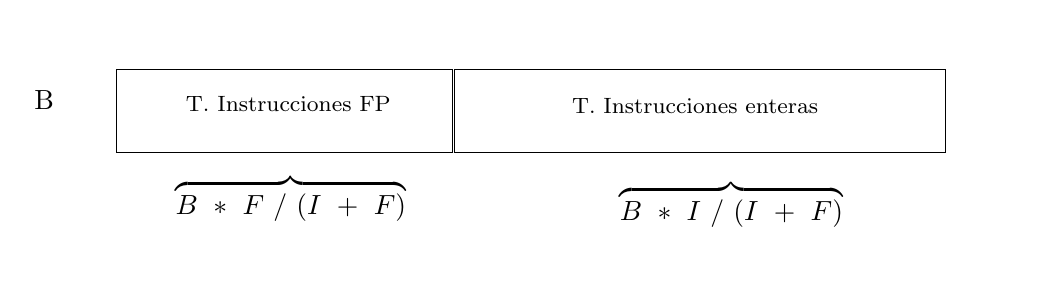
\begin{tikzpicture}[x=0.75pt,y=0.75pt,yscale=-1,xscale=1, baseline=(XXXX.south) ]
\path (0,109);\path (483,0);\draw    ($(current bounding box.center)+(0,0.3em)$) node [anchor=south] (XXXX) {};
%Shape: Rectangle [id:dp446170275508015] 
\draw   (43,20) -- (204.5,20) -- (204.5,60) -- (43,60) -- cycle ;
%Shape: Rectangle [id:dp30899223371026585] 
\draw   (205.5,20) -- (442,20) -- (442,60) -- (205.5,60) -- cycle ;
% Text Node
\draw (261,33) node [anchor=north west][inner sep=0.75pt]   [align=left] {{\footnotesize T. Instrucciones enteras}};
% Text Node
\draw (75,32) node [anchor=north west][inner sep=0.75pt]   [align=left] {{\footnotesize T. Instrucciones FP}};
% Text Node
\draw (2,29) node [anchor=north west][inner sep=0.75pt]   [align=left] {B};
% Text Node
\draw (70,69) node [anchor=north west][inner sep=0.75pt]   [align=left] {$\displaystyle \overbrace{B\ *\ F\ /\ ( I\ +\ F)}$};
% Text Node
\draw (284,72) node [anchor=north west][inner sep=0.75pt]   [align=left] {$\displaystyle \overbrace{B\ *\ I\ /\ ( I\ +\ F)}$};
\end{tikzpicture}

%
\end{frame}

\begin{frame}
\frametitle{MFLOPS}
Podemos pensar el denominador como $T_{ex\_fp} = B - B_{enteras}$, donde $B_{enteras}$ representa la fracción 
de tiempo durante la cuál se ejecutan instrucciones enteras, siendo $B_{enteras} = \sfrac{I}{(I+F)} \times B $
%
\medskip
\begin{displaymath}
MFLOPS = \frac{F}{B \times (1 - \sfrac{I}{(I + F)}) \times 10^6} = \frac {I + F}{B \times 10^6}  = 80
\end{displaymath}
\end{frame}

\begin{frame}
\frametitle{Un colega quiere comprar el coprocesador a pesar que tiene una tasa de MIPS inferior al uso del procesador
unicamente ¿Tiene razón? Justificar la respuesta}

Si, tiene razón.\\
\medskip
La métrica que determina el desempeño de un sistema es el tiempo de ejecución. Si comparamos el tiempo de ejecutar
el benchmark al utilizar el coprocesador ($B$) con respecto a simular a través de operaciones enteras ($W$), el 
\textit{Speed up} obtenido es de aproximadamente $3.6$

\bigskip
Entonces, ¿Qué significa que $MIPS_{e}$ sea mayor que $MIPS_{c}$
\end{frame}

\begin{frame}

La ejecución en ambos sistemas no es equivalente. La versión que carece del coprocesador debe ejecutar un número extra
de instrucciones por cada instrucción de punto flotante ($Y$).\\ 
\medskip
Esta cantidad desproporcionada de instrucciones destinadas a la emulación de punto flotante es lo que causa que 
$MIPS_{e}$ sea mayor que $MIPS_{c}$\\
\medskip
En definitiva, la ejecución de un número mucho mayor de instrucciones incrementa el tiempo de ejecución junto con
la tasa de MIPS: $IC_{e} >> IC_{c} $
\end{frame}
%
\end{document}
